\section{Our Approach}
\label{sec:approach}

% latex problem -- this figure should be displayed near the section approach
\begin{figure*}[t]
  \centering
  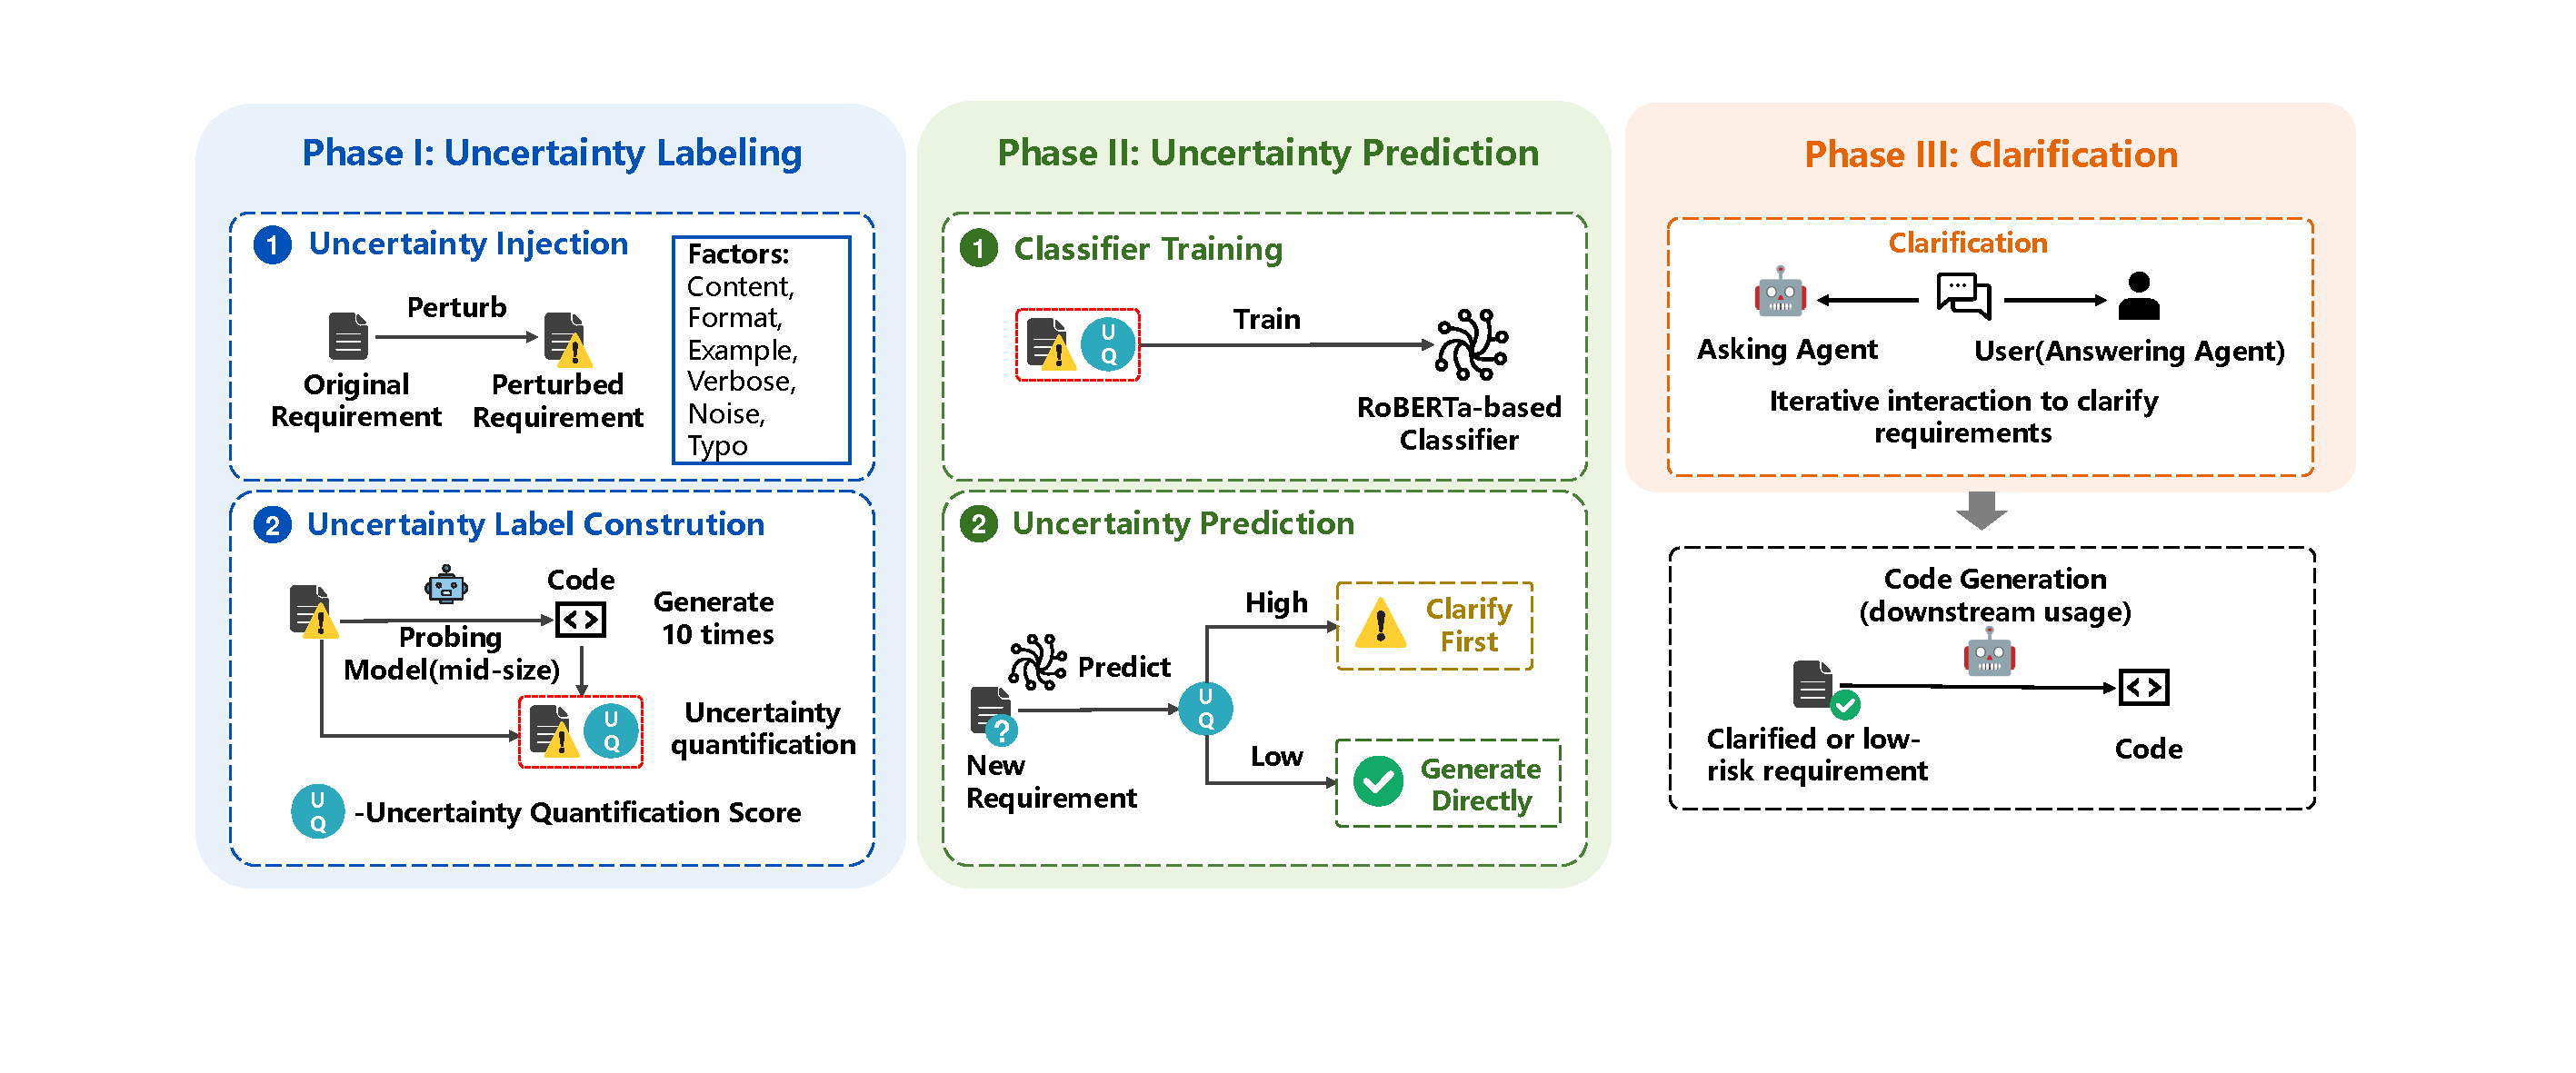
\includegraphics[trim={2cm, 3.5cm, 4.5cm, 1.5cm}, clip, width=0.95\textwidth]{overview.pdf}
  \caption{Overview of our approach \textsc{Pulse}.}
  \label{fig:approach-figure}
\end{figure*}

Figure~\ref{fig:approach-figure} illustrates the workflow of our approach, \textsc{Pulse}, which consists of three stages: requirement uncertainty labeling, requirement uncertainty prediction, and uncertainty-aware clarification. In Stage I, we inject perturbation types that affect code generation reliability (see Section~\ref{sec:preStudy}) into benchmark requirements. Inspired by Expert-Novice Differences~\cite{Chi1981ExpertNovice} and schema-theoretic default reasoning~\cite{Rumelhart1980Schemata}, we use a moderate-sized model, Qwen2.5-7B-Coder-Instruct, to annotate requirements prone to unreliable generation, following the uncertainty metric in Section~\ref{sec:preStudy}. In Stage II, the resulting $UQ$ scores are transformed into binary labels to train a lightweight RoBERTa-based classifier. Given a requirement, the classifier estimates the probability that the requirement belongs to the high-uncertainty class, thereby enabling efficient pre-generation assessment without repeated generation. In Stage III, the predicted uncertainty label drives intervention: uncertainty-prone requirements undergo clarification before generation, while low-risk ones proceed directly. To enable scalable evaluation, we implement a multi-agent simulation of clarification dialogues between a code generator and a user.

\subsection{Requirement Uncertainty Labeling}

We adopt the uncertainty injection setup from Section~\ref{sec:preStudy}. This section then details the selection of the probe model and the UQ-based binary labeling process.

\subsubsection{Uncertainty Probe Model}

Requirement uncertainty labeling relies on repeated generation to observe whether a requirement induces stable or unstable high-quality code generation outcomes. Since our goal is to label uncertainty that can lead to unreliable code generation across multiple runs and models, the choice of the generator model is critical: different models may exhibit different sensitivity to the same requirement perturbation, and the label should largely reflect model-agnostic uncertainty.

We use a moderate-sized code generation model as the uncertainty probe. According to Expert-Novice Differences~\cite{Chi1981ExpertNovice} and schema-theoretic default reasoning~\cite{Rumelhart1980Schemata}, we reason that frontier models tend to automatically clarify uncertain requirements. As a result, they compress both functional instability and structural divergence, making requirements that appear clear to expert models potentially uncertain for other models. In contrast, a moderate-sized model retains good capability in requirement interpretation while being more sensitive to requirement variations. 

We empirically verify this reasoning with a simple evaluation. Table~\ref{tab:model_selection} compares generation reliability and uncertainty across models of different capacities. On HumanEval-ET, DeepSeek-V3.2 achieves a slightly higher APR than Qwen2.5-7B-Coder-Instruct\cite{hui2024qwen2.5} while producing a much smaller mean UQ score. Similar trends can also be observed on MBPP-ET. These results suggest that stronger models may mask requirement-induced uncertainty through more stable generation, whereas a moderate-sized model can better expose variation in generation consistency. Therefore, we use Qwen2.5-7B-Coder-Instruct as the uncertainty probe for constructing UQ-based labels.

\begin{table}[t]
\vspace{0.5em}
\centering
\caption{Effect of model capacity on generation reliability and uncertainty. APR denotes Average Pass Rate and UQ denotes Mean Uncertainty Score.}
\label{tab:model_selection}
\footnotesize
\setlength{\tabcolsep}{4pt}
\begin{tabular*}{\columnwidth}{@{\extracolsep{\fill}}llll@{}}
\hline
Dataset & Model & APR & UQ \\
\hline
HumanEval-ET & DeepSeek-V3.2 & 0.844 & 0.057 \\
HumanEval-ET & Qwen2.5-7B-Coder-Instruct & 0.807 & 0.154 \\
MBPP-ET & DeepSeek-V3.2 & 0.527 & 0.148 \\
MBPP-ET & Qwen2.5-7B-Coder-Instruct & 0.493 & 0.255 \\
\hline
\end{tabular*}
\end{table}

\subsubsection{UQ-based Binary Labeling}

Following the UQ metric defined in Section~\ref{sec:preStudy}, we assign each requirement instance a model-centered uncertainty score based on repeated generation inconsistency. Specifically, for each requirement $r$, we repeatedly sample $K=10$ generated programs from the uncertainty probe model and evaluate them against the corresponding test suite. The resulting UQ score summarizes the degree to which repeated generations are inconsistent in terms of functional outcomes and implementation structures.

To support requirement uncertainty prediction, we need binary supervision labels indicating whether a requirement should be treated as high-uncertainty. While Stage I produces a continuous UQ score instead of a discrete class label. To obtain supervision for classifier training, we convert the continuous UQ score into a binary label using a two-component Gaussian Mixture Model (GMM)~\cite{bishop2006pattern}. Instead of applying a manually fixed threshold to the continuous UQ scores, we use GMM to derive data-driven labels based on the empirical distribution of UQ scores. This makes our label construction less dependent on hand-tuned thresholds and, more importantly, allows our method to automatically adapt to different datasets without requiring dataset-specific calibration. GMM-based soft grouping has also been adopted in recent uncertainty quantification studies to model latent structures in generated outputs~\cite{luo2026agsc}.

In our setting, each requirement $r$ is associated with a continuous uncertainty score $U(r)$ computed in Stage I. The GMM treats the distribution of $U(r)$ as a mixture of two latent components, corresponding to low-risk and high-uncertainty requirements. We fit the GMM using the classical EM algorithm~\cite{dempster1977maximum}. After fitting the mixture model, we assign the component with the larger mean UQ score to the high-uncertainty class. Let $z$ denote the latent component assignment and let $z=1$ represent the high-uncertainty component. We then define the binary uncertainty label $y(r)$ according to the GMM posterior probability:
\begin{equation}
\label{eq:gmmLabel}
y(r)=
\begin{cases}
1, & P_{\mathrm{GMM}}(z=1 \mid U(r)) \geq 0.5,\\
0, & P_{\mathrm{GMM}}(z=1 \mid U(r)) < 0.5,
\end{cases}
\end{equation}
where $P_{\mathrm{GMM}}(z=1 \mid U(r))$ denotes the posterior probability estimated by the fitted GMM. This probability is used only for label construction, whereas the classifier later predicts $p(y=1\mid r)$ directly from the requirement text.

The resulting binary labels serve as supervision signals for training the requirement uncertainty classifier in Stage II. In this way, repeated generation is only used offline to construct model-centered labels, while the trained classifier enables direct uncertainty assessment from requirement text at inference time.

\subsection{Requirement Uncertainty Prediction}

%Requirement uncertainty labeling provides model-centered supervision signals for identifying requirements that are likely to induce unreliable generation. However, computing UQ scores requires repeated code generation and test execution, which is costly for pre-generation assessment. 
We train a lightweight classifier that estimates requirement uncertainty directly from requirement text.


\subsubsection{Problem Formulation}
Given a natural language requirement $r$, our objective is to predict whether it belongs to the high-uncertainty class without performing repeated code generation. Based on the binary labels $y(r)$ constructed above, we train an uncertainty prediction model $f(\cdot)$ that maps $r$ to the probability of the high-uncertainty class:
\begin{equation}
\label{eq:uncertaintyPrediction}
f(r) \rightarrow p(y=1 \mid r),
\end{equation}
where $p(y=1 \mid r)$ denotes the classifier-predicted probability that requirement $r$ belongs to the high-uncertainty class. Since the classifier output is a continuous probability, it must be converted into a binary decision before being used as a clarification trigger. A fixed threshold of $0.5$ assumes that classifier scores are well calibrated and that the two classes have balanced decision costs, which may not hold in our setting. In particular, high-uncertainty requirements are the primary targets for clarification, and missing such cases may prevent potentially beneficial clarification from being triggered. Therefore, following threshold-selection practice for optimizing classification decisions~\cite{lipton2014optimal}, we select a decision threshold $\tau$ on the validation set and choose the threshold that maximizes the validation objective for identifying high-uncertainty requirements. The resulting binary prediction is defined as:
\begin{equation}
\label{eq:predictionLabel}
\hat{y}(r)=
\begin{cases}
1, & p(y=1 \mid r) \geq \tau,\\
0, & p(y=1 \mid r) < \tau,
\end{cases}
\end{equation}
where $\hat{y}(r)=1$ indicates that the requirement is predicted as high-uncertainty and should trigger uncertainty-aware clarification, while $\hat{y}(r)=0$ indicates that the requirement is treated as low-risk.


\subsubsection{Classifier Training}
%To enable efficient requirement uncertainty prediction, 
We adopt RoBERTa~\cite{liu2019roberta} as the backbone text encoder and attach a lightweight binary classification head. 
We select RoBERTa because it provides strong contextual text representations for natural language understanding tasks while remaining substantially more lightweight than generation models, making it suitable for efficient pre-generation uncertainty prediction~\cite{liu2019roberta,devlin2019bert}. 
Given a requirement description, the encoder maps the input text into contextualized representations, which are then passed to the classification head to estimate the probability that the requirement belongs to the high-uncertainty class.
The trained classifier enables the determination of whether a given requirement description exhibits uncertainty.


\subsection{Uncertainty-aware Clarification}
Requirements with high uncertainty are flagged for clarification, while low-risk ones are directly used for code generation. The clarification itself can be handled by external methods. In this work, inspired by human–AI interaction, we design a simple multi-agent clarification framework (Figure~\ref{fig:approach-figure}). It consists of an asking agent that initiates clarification questions and an answering agent that simulates user responses.

The asking agent targets issues that may undermine reliable code generation, such as ambiguity, underspecification, inconsistency, and missing constraints. To keep questions actionable, it focuses on implementation-relevant details like edge cases, I/O types, error handling, performance, and missing context, rather than posing generic queries.

To control cost, the process is bounded by a maximum number of rounds and can terminate early when further dialogue yields no actionable information. After the ask–answer loop, \textsc{Pulse} consolidates the confirmed information into a clarified requirement. Instead of rewriting, we keep the original requirement as the main specification and attach each clarification in the form of \emph{[original requirement] + [1. clarified info] + [2. clarified info] + ....} This provenance-aware formulation is inspired by prior work that refines ambiguous requirements based on additional evidence rather than arbitrary rewriting~\cite{mu2024clarifygpt,jia2025specfix}, helping avoid semantic drift while still making implicit details explicit for downstream code generation.
